\documentclass[a4paper,11pt]{report}

\usepackage{amsmath}
\usepackage{amsthm}
\usepackage{fullpage}
\usepackage{tikz}

\usetikzlibrary{graphs,graphs.standard}

\makeatletter
\pgfmathdeclarefunction{alpha}{1}{%
  \pgfmathint@{#1}%
  \edef\pgfmathresult{\pgffor@alpha{\pgfmathresult}}%
}

\usepackage{bussproofs}
\usepackage{mathpartir}
\usepackage{prooftrees}
\usepackage{color}

\newcommand*{\contract}[2]{contraction of $#1$ with $#2$}

\newcommand*{\MP}{Modus Ponens }
\newcommand*{\MPr}[2]{\MP of \ref{#1} and \ref{#2}}

\author{Sylvain Julmy}
\date{\today}

\setlength{\parindent}{0pt}

\begin{document}

\begin{center}
  \Large{
    Mathematical Methods for Computer Science 2\\
    Spring 2018
  }
  \noindent\makebox[\linewidth]{\rule{\linewidth}{0.4pt}}

  Series 13
  \vspace*{1.4cm}

  Sylvain Julmy
  
  \noindent\makebox[\linewidth]{\rule{\linewidth}{0.4pt}}
\end{center}

\section*{\texttt{1}}

\subsection*{\texttt{a)}}

$L = \{a^ib^jc^k | i < j < k\}$ is not context-free :

Assume $L$ is context-free, then the Pumping Lemma hold, then for all $\omega
\in L$, we have $\omega = uvwxy$ such that $vx \neq \epsilon, |vwx| \leq p$ and
$i \geq 0, uv^iwx^iy$.

We pick $z$ as $a^{m+2}b^{m+1}c^{m}$, where $m$ is the pumping length. $z$ is
clearly in $L$ and $|z| \geq m$. We know that $|vwx| \leq m$ and $|vx| > 0$,
then we know that $vwx$ must consist of :

\begin{enumerate}
\item only $a$'s $\implies vx = a^s$ since the lemma tell us $|vx| > 0$. Now we
  take $i=0$, then we have $z' = uv^0wx^0y \in L$ but $z'$ is
  $a^{m+2-s}b^{m+1}c^{m}$ and since $s > 0$, the pumping lemma don't hold.
\item some $a$'s and some $b$'s $\implies vx = a^sb^t$ such that $s+t > 0$, we
  take $i=0$ then $z'$ is in the form $a^{m+2-s}b^{m+1-t}c^m$. If $t$ is
  positive, then $|b| > |c|$ and its not in the language. If $t = 0$, then its
  case $1$.
\item only $b$'s take $i = 0$, then $z'$ is in the form $a^{m+2}b^{m+1-s}c^{m}$
  and $s$ is positive, which violates the condition that $|b| > |c|$. So $z'
  \not\in L$.
\item some $b$'s and some $c$'s : take $i = 2$ then $z' =
  a^{m+2}b^{m+1+s}c^{m+t}$, if $s \neq 0$ then $|a| > |b|$ don't hold. If $s
  \neq 0$ then $t \neq 0$ then $|b| > |c|$ don't hold, so $z' \not\in L$.
\item only $c$'s : take $i=2$, then $z' = a^{m+2}b^{m+1}c^{m+s}$, since $s$ is
  positive, then $|b| > |c|$ don't hold.
\end{enumerate}

Since all five cases fail to pump, the Pumping Lemma tells us that this language
is not context-free.

\subsection*{\texttt{b)}}

$\{a^i | i \text{ is a prime} \}$ is not context-free :

Let $v=x^q$ and $y = x^t$, note that the Pumping Lemma requires $q+t>0$. Let
$r=|uxz|=p−q−t$. Then $|uvrxyrz|=r+rq+rt=r(1+q+t)$ is divisible by both $r$ and
$1+q+t>1$ and thus is not prime as long as $r>1$.

Then there are two unsettled cases: if $r=0$, $|uv2xy2z|=|v2y2|=2p$ is not
prime. Finally, if $r=1$,
$|uvp+1xyp+1pz|=1+(p+1)q+(p+1)t=1+(p+1)(q+t)=1+(p+1)(p−1)=p2$ isn't prime.

\section*{\texttt{2}}

The language $L = \{0^i1^j0^{i+j}\}$ is not regular :

Assume $L$ is regular, let $\omega = 0^s1^t0^{t+s}$. Thus $|\omega| = 2(s+t)$,
by the pumping lemma, let $\omega = xyz$, where $|xy| \leq n$. Let $x = 0^p$, $y
= 0^q$ and $z = 0^r1^t0^{p+q+r+t}$ where $p + q + r = s$, $p \neq 0$, $q \neq
0$, $r \neq 0$. Thus $|y| \neq 0$. Let $k = 2$, then $xy^2z =
0^p0^{2q}0^r1^t0^{p+2q+r+t}$. Then the number of $a$ is $2(p + 2q + r) = 2(n +
q)$. Hence $xy^2z = 0^p0^{2q}0^r1^t0^{n+q+t}$, since $q \neq 0$ $xy^2z$ is not
of the form $0^i1^j0^{i+j}$, thus $xy^2z \not\in L$, hence $L$ is not regular.

The language $L = \{0^i1^j0^{i+j}\}$ is context-free since the following grammar
generate it:
\begin{align*}
  A &\to 0AB0\ |\ \epsilon \\
  B &\to 1B0\ |\ \epsilon
\end{align*}

\section*{\texttt{3}}

\section*{\texttt{4}}

If $L$ is context-free, then there is a PDA $P$ accepting it. If $M$ is regular,
then there is a DFA $F$ accepting it. The intersection of $L$ and $M$ is the
language that accept word that are in $L$ and in $M$. Any word that are in the
intersection are accepted by $D$ but not all the word that are accepted by $D$,
only those accepted by $P$.

The cross product proof consists of constructing an automaton $P \otimes F$
which contains the mechanics of both $P$ and $F$, and which accepts only words for
which both sides accept. The cross-product automaton is a PDA (and therefore the
recognized language is context-free) — intuitively, because the cross product
with an $n$-state DFA consists of taking $n$ copies of $P$ and adding
$(q,a,[q])$ arrows between matching states in $P$ where the DFA has a arrows.
The result is not a finite automaton in general (not even a non-deterministic
one) because the $P$ part relies on the stack and this reliance does not go away
in $P \otimes F$ in general.

\section*{\texttt{5}}

\subsection*{\texttt{a)}}

The language generated is finite because there are no cycle in the following
graph of possible generation :

\begin{center}
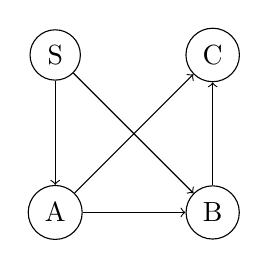
\begin{tikzpicture}
  \node[shape=circle,draw=black] (s) at (0,2) {S};
  \node[shape=circle,draw=black] (a) at (0,0) {A};
  \node[shape=circle,draw=black] (b) at (2,0) {B};
  \node[shape=circle,draw=black] (c) at (2,2) {C};

  \draw[->] (s) to node [above] {}  (a);
  \draw[->] (s) to node [above] {}  (b);
  \draw[->] (a) to node [above] {}  (b);
  \draw[->] (a) to node [above] {}  (c);
  \draw[->] (b) to node [above] {}  (c);
\end{tikzpicture}
\end{center}

\subsection*{\texttt{b)}}

The language generated is infinite  because we have a cycle between $C$ and $S$
:

\begin{center}
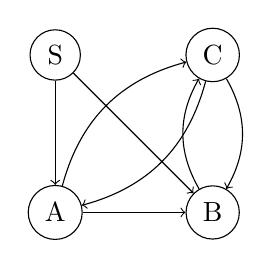
\begin{tikzpicture}
  \node[shape=circle,draw=black] (s) at (0,2) {S};
  \node[shape=circle,draw=black] (a) at (0,0) {A};
  \node[shape=circle,draw=black] (b) at (2,0) {B};
  \node[shape=circle,draw=black] (c) at (2,2) {C};

  \draw[->] (s) to node [above] {}  (a);
  \draw[->] (s) to node [above] {}  (b);
  \draw[->] (a) to node [above] {}  (b);
  \draw[->] (a)[bend left] to node [above] {}  (c);
  \draw[->] (b)[bend left] to node [above] {}  (c);
  \draw[->] (c)[bend left] to node [above] {}  (a);
  \draw[->] (c)[bend left] to node [above] {}  (b);
\end{tikzpicture}
\end{center}

The following familly of word is in $L$ :

\begin{gather*}
  S \to
  AB \to
  BCB \to
  BABB \to
  BACCB \to
  BAABCB \to \\
  BAACCCB \to
  BAAABCCB \to
  BAAACCCCB \to \\
  BAAAABCCCB \to
  BAAAACCCCCB \to
  BAAAAABCCCCB \to
  \dots
\end{gather*}

all the words of the form $ba^nbb^nb = ba^nb^{n+2}$.

\end{document}
